\subsection{Results}
Here, the process that a curve undergoes from initialisation to the generation of the final final velocity profile will be demonstrated, drawing upon the theoretical underpinnings of the previous sections.
Firstly, a curve is obtained through plotting or by extraction from image features. The curve that will be taken through the optimisation process can be seen in Figure \ref{fig:example}. The curve has seven control points and has a complex shape that will incur several changes in the limiting axis, demonstrating the ability of our optimisation process to drive the machine to the limits of its physical limitations.

\begin{figure}[htbp]  
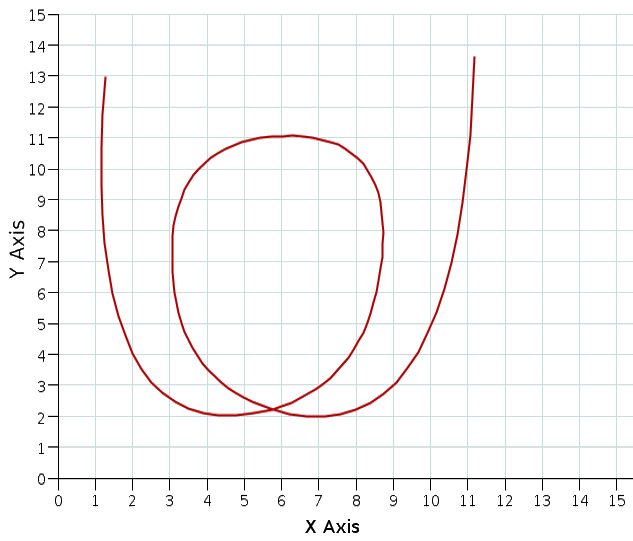
\includegraphics[width=0.7\textwidth]{figures/optimisation/exampleSpline.png}
\caption[Optimisation example curve]{ This spline has 7 control points and 10 knots. This example will be used to demonstrate the properties of URBS curves and the optimisation process.
\label{fig:example}}
\end{figure}
\clearpage

The spline is decomposed into its X and Y axis coordinates, giving the positions that each axis should achieve at each point on the curve. The result of these parametrisations can be seen in Fig.\ref{fig:xy_s}. Bundled onto the same graph with these curves is the simulated final product of the optimisation and transmission process. It can be seen that the black curve representing the final theoretical output at this level of zoom has an error that is nearly imperceptible. The deviation that is discernible from the correct path is not an artefact of the optimisation process. The velocity profile sampling which is required to pass the movement information across to the plant discretises the velocity information, which causes accumulating integration error.\footnote{Further work would include an interpolation scheme based on the sampling rate that would adjust these profiles such that the machine would be back on the curve after each sampling period. This implementation is not trivial as the adjustments to the velocity discretisation may cause the acceleration constraints to become exceeded.} However it can be seen in Fig.\ref{fig:xy_s} that the final effect is slight. These effects are also reset at the culmination of each curve. Thus the introduced error was considered to be within allowable bounds for our purposes.

\begin{figure}[htbp]
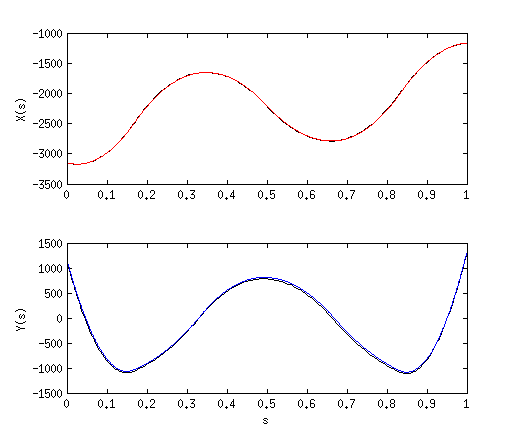
\includegraphics[width=\textwidth]{figures/optimisation/xy_s.png}
\caption[Indexed curve position and theoretical final path]{
The X axis (TOP) and Y axis (BOTTOM) displaying the correct trajectory in colour and the approximated path that will be followed in black, given a velocity profile that is sampled at 25Hz.
\label{fig:xy_s}}
\end{figure} 

The discretisation aspect discussed in previous sections mentioned that the problem required a discrete approximation of the derivatives of the given path. The URBS curve used can easily have the parametrised curve derivatives ($\textbf{q}'(t)$ and $\textbf{q}''(t)$) extracted at each discretisation point for the SeDuMi solver. The curves for the first and second derivatives of the axis position with respect to the parametrisation variable for the path in the example spline seen in Fig~\ref{fig:example} can be seen in Fig~\ref{fig:xy_dds_ds}. These values are extracted by taking the derivative of the quadratic URBS weighting equations with respect to the parametrisation variable $s$.
Unsurprisingly the first derivative is piecewise linear and continuous. Thus, it is quite easy to find the maximum value for a given discrete section and thus encode the discrete approximation with the requisite path parameters.
The second derivative is piecewise linear. Finding something that would be considered a limiting value over a discrete path section is a little troublesome here, as the value can jump to differing discrete states. This issue can actually cause the discrete approximation of the constraints to be invalid for low sampling values, as will be discussed later.

\begin{figure}[htbp]
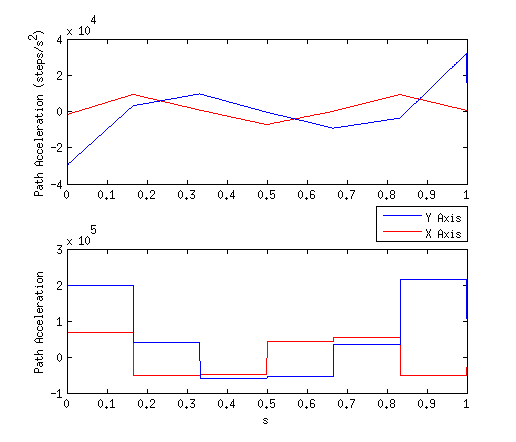
\includegraphics[width=\textwidth]{figures/optimisation/xy_dds_ds.png}
\caption[Parametrised curve derivatives]{
The first (TOP) and second (BOTTOM) derivatives of the parametrised curve position for the example curve. Note the discrete jumps in level for the second derivative and the corresponding changes in gradient for the first derivative.
\label{fig:xy_dds_ds}}
\end{figure}

Given that we have discretised and found the corresponding constraints to complete the construction of the problem, the solver SeDuMi can compute the discrete $\dot{s}^*(s)$, which is the approximated time optimal trajectory. The trajectory which was arrived at for the given example curve can be seen in Fig.~\ref{fig:sdot_st}.
The final calculation step in order to achieve the desired $s^*(t)$ requires that we compute the resulting time $t$ for each $s(s)$ via the inverse relation
\begin{align*}
t(s) &= \int_0^s\frac{1}{\dot{s}^*(s)}du\\ 
\end{align*}

\begin{figure}[htbp]
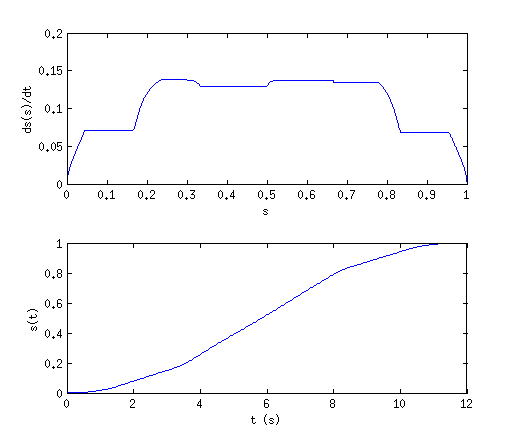
\includegraphics[width=\textwidth]{figures/optimisation/sdot_st.png}
\caption[$\dot{s}^*(s)$ and $s^*(t)$]{
The optimal curve velocity (TOP) and the retrieved path trajectory (BOTTOM) for the example curve.
\label{fig:sdot_st}}
\end{figure}

Since $\dot{s}^*(s)$ is defined in a piecewise non-linear fashion due to its direct relation to the piecewise linear trajectory $b(s)$, we obtain a mapping between $t$ and $s$ for arbitrary $t$ via the algorithm outlined in Appendix C. The output $s(t)$ can be seen in Fig.~\ref{fig:sdot_st}. Though the solution can be solved for a piecewise closed form, an algorithm that solves for a given discrete sampling rate $k\Delta T$ was used instead. This allows us to specify an arbitrary desired velocity sampling frequency and hence use the subsequently calculated values of $s(k\Delta T)$ to generate the sampled velocity profile via 
\begin{align*}
\frac{d\textbf{q}\left(k \Delta T\right)}{dt} &= \frac{\textbf{q}\left(s(k\Delta T)\right)}{ds}\frac{ds(k\Delta T)}{dt}
\end{align*}
Hence, we have generated the optimal axis velocity curves that can be sent to the unit in order to faithfully follow a URBS curve with a time optimal trajectory.
An output of the optimal trajectory $\dot{\textbf{q}}(k\Delta T)$ and $\ddot{\textbf{q}}(k\Delta T)$ can be seen in Fig.~\ref{fig:bangbang}.

\begin{figure}[htbp]
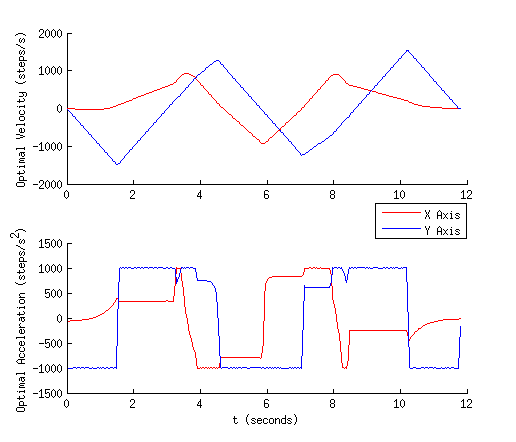
\includegraphics[width=\textwidth]{figures/optimisation/bangbang_xy_ddt_dt.png}
\caption[$\dot{\textbf{q}}^*(t)$ and $\ddot{\textbf{q}}^*(t)$]{
The optimal axis velocity (TOP) and the optimal path acceleration (BOTTOM) for the example curve.
\label{fig:bangbang}}
\end{figure}